% Quick start guide
\documentclass[aspectratio=169]{beamer}

\usepackage{caption}
\usepackage{subcaption}
\usepackage{minted}

\usetheme {default}


\setbeamertemplate{itemize items}[square]
\setbeamertemplate{navigation symbols}{}

% Title page details
\title{Introduction to Overleaf}
\subtitle{Learning how to use Overleaf and \LaTeX{}}
\author{Marcelo Garcia}
\institute{KAUST Library}
\date{}

\logo{
\includegraphics[width=3cm]{images/KAUST_Logo_Black.png}} 

\begin{document}

\begin{frame}
% Print the title page as the first slide
\titlepage
\end{frame}

%
% Table of contents (TOC)
%
% \begin{frame}{Outline}
%     \tableofcontents    
% \end{frame}

% \section{Overleaf and \LaTeX{}}
% \section{Text Processor vs Text Editor}
% \section{\LaTeX{} and MS-Word}
%
% End of TOC.
%

\begin{frame}{Overleaf and \LaTeX{}}
Overleaf in their own words: ``Overleaf is a startup and social enterprise that builds modern collaborative authoring tools for scientists — like \textit{Google Docs for Science}. Our primary product is an online, real time collaborative editor for papers, theses, technical reports and other documents written in the \textit{LaTeX markup language}.''

Sounds good, but what is \emph{LaTeX markup language}?
\end{frame}

\begin{frame}[fragile]
\frametitle{Text Processor vs Text Editor}

\begin{columns}[c]

    \begin{column}{.5\textwidth}
    \small
\begin{verbatim}
<!DOCTYPE html>
<html>
<head>
<title>Page Title</title>
</head>
<body>

<h1>This is a Heading</h1>
<p>This is a paragraph.</p>

</body>
</html> 
\end{verbatim}
    \normalsize
    \end{column}

    \begin{column}{.5\textwidth}
    \begin{figure}
        \centering
        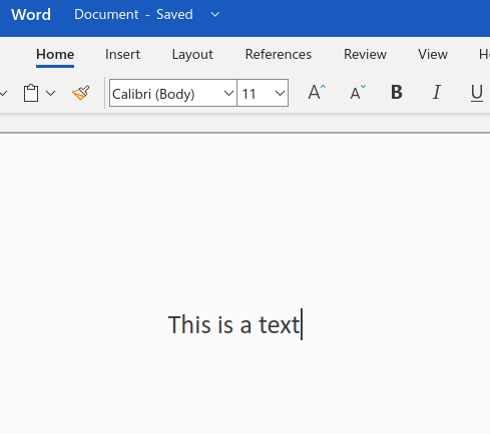
\includegraphics[width=0.9\textwidth]{images/ms_word_picture.png}
    \end{figure}
    \end{column}

\end{columns}
\end{frame}

\begin{frame}{\LaTeX{} and MS-Word}
    Why to consider \LaTeX{} over Word?
    \begin{figure}
        \centering
        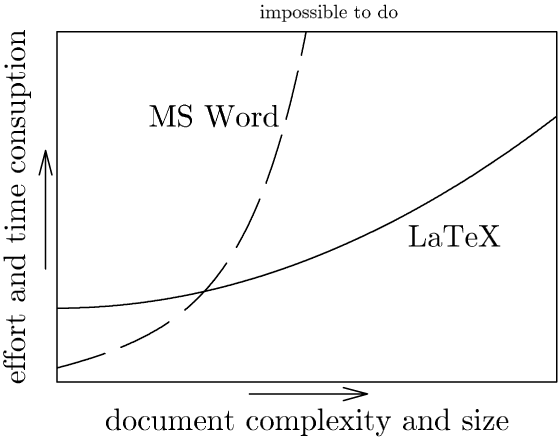
\includegraphics[scale=0.4]{images/miktex.png}
        %\caption{Caption}
        \label{fig:latex_word_pain}
    \end{figure}
\end{frame}

\begin{frame}{Origins of \LaTeX}
    \begin{columns}
    \small
    \begin{column}{0.8\textwidth}
        Donald E. Knuth created $\tau \varepsilon \chi$ (Tau Epsilon Chi) between 1977 and 1979.
        \begin{itemize}
            \item Unhappy how his book looked after publisher changed from hot metal typesetting (19th century tech) to phototypesetting in 1960s.
            \item Greek word ``Tekne'' means "art, skill, craft in work," and it's the root for the word ``technology.''
        \end{itemize}
    \end{column}
            
    \begin{column}{0.2\textwidth}
        \begin{figure}
        \centering
            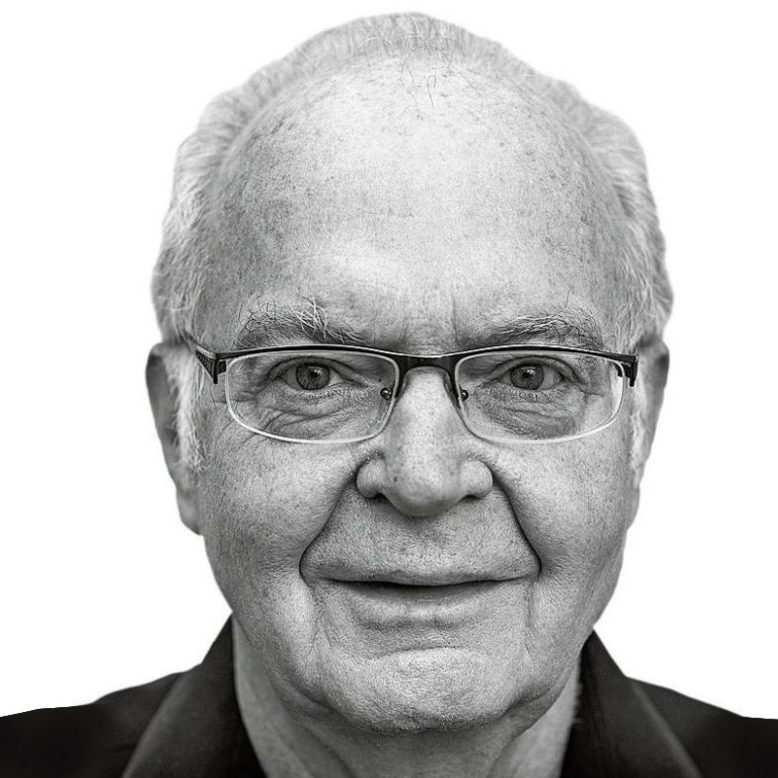
\includegraphics[scale=0.06]{images/donald-knuth.jpg}
        \end{figure}
    \end{column}
    \normalsize                
    \end{columns}

    \begin{columns}
        \begin{column}{0.7\textwidth}
        \end{column}
        \begin{column}{0.3\textwidth}
        \end{column}
    \end{columns}

    \begin{columns}
    \small
    \begin{column}{0.8\textwidth}
        Leslie Lamport extended TeX
        \begin{itemize}
            \item While using TeX he noticed could expand with macros
            \item Released his LaTeX macros between 1984 and 1985. He handed the control of \LaTeX{} in 1989.
        \end{itemize}
    \end{column}
            
    \begin{column}{0.2\textwidth}
        \begin{figure}
        \centering
            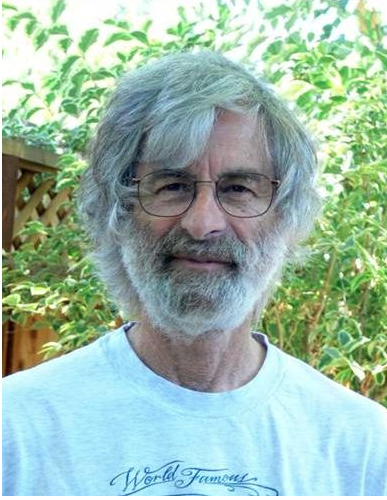
\includegraphics[scale=0.12]{images/LeslieLamport_2.jpg}
        \end{figure}
    \end{column}
    \normalsize                
    \end{columns}

\end{frame}

\begin{frame}{Logging in Overleaf}
    \begin{columns}[c]
        \begin{column}{.5\textwidth}
            \begin{figure}
                \centering
                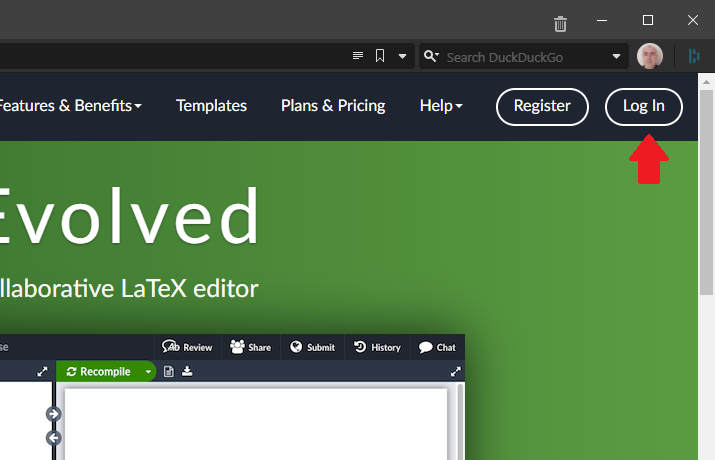
\includegraphics[scale=0.27]{images/overleaf_login.png}
            \end{figure}      
        \end{column}

        \begin{column}{.5\textwidth}
            \begin{figure}
                \centering
                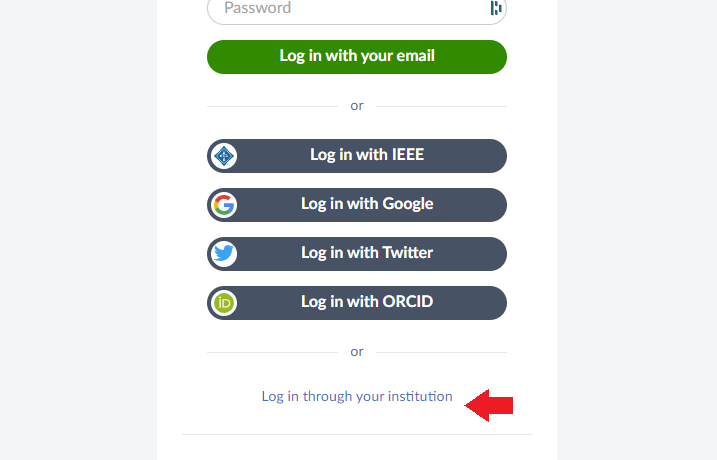
\includegraphics[scale=0.27]{images/overleaf_login_institution.png}
            \end{figure}
        \end{column}
    \end{columns}

    You will need your KAUST credentials for the login.
\end{frame}

\begin{frame}{Projects Overview}
    ``Home'' page of the account. You will return to this page, if explore the online help from Overleaf, and decide to return to your projects. It's a shortcut.
    \begin{figure}
        \centering
        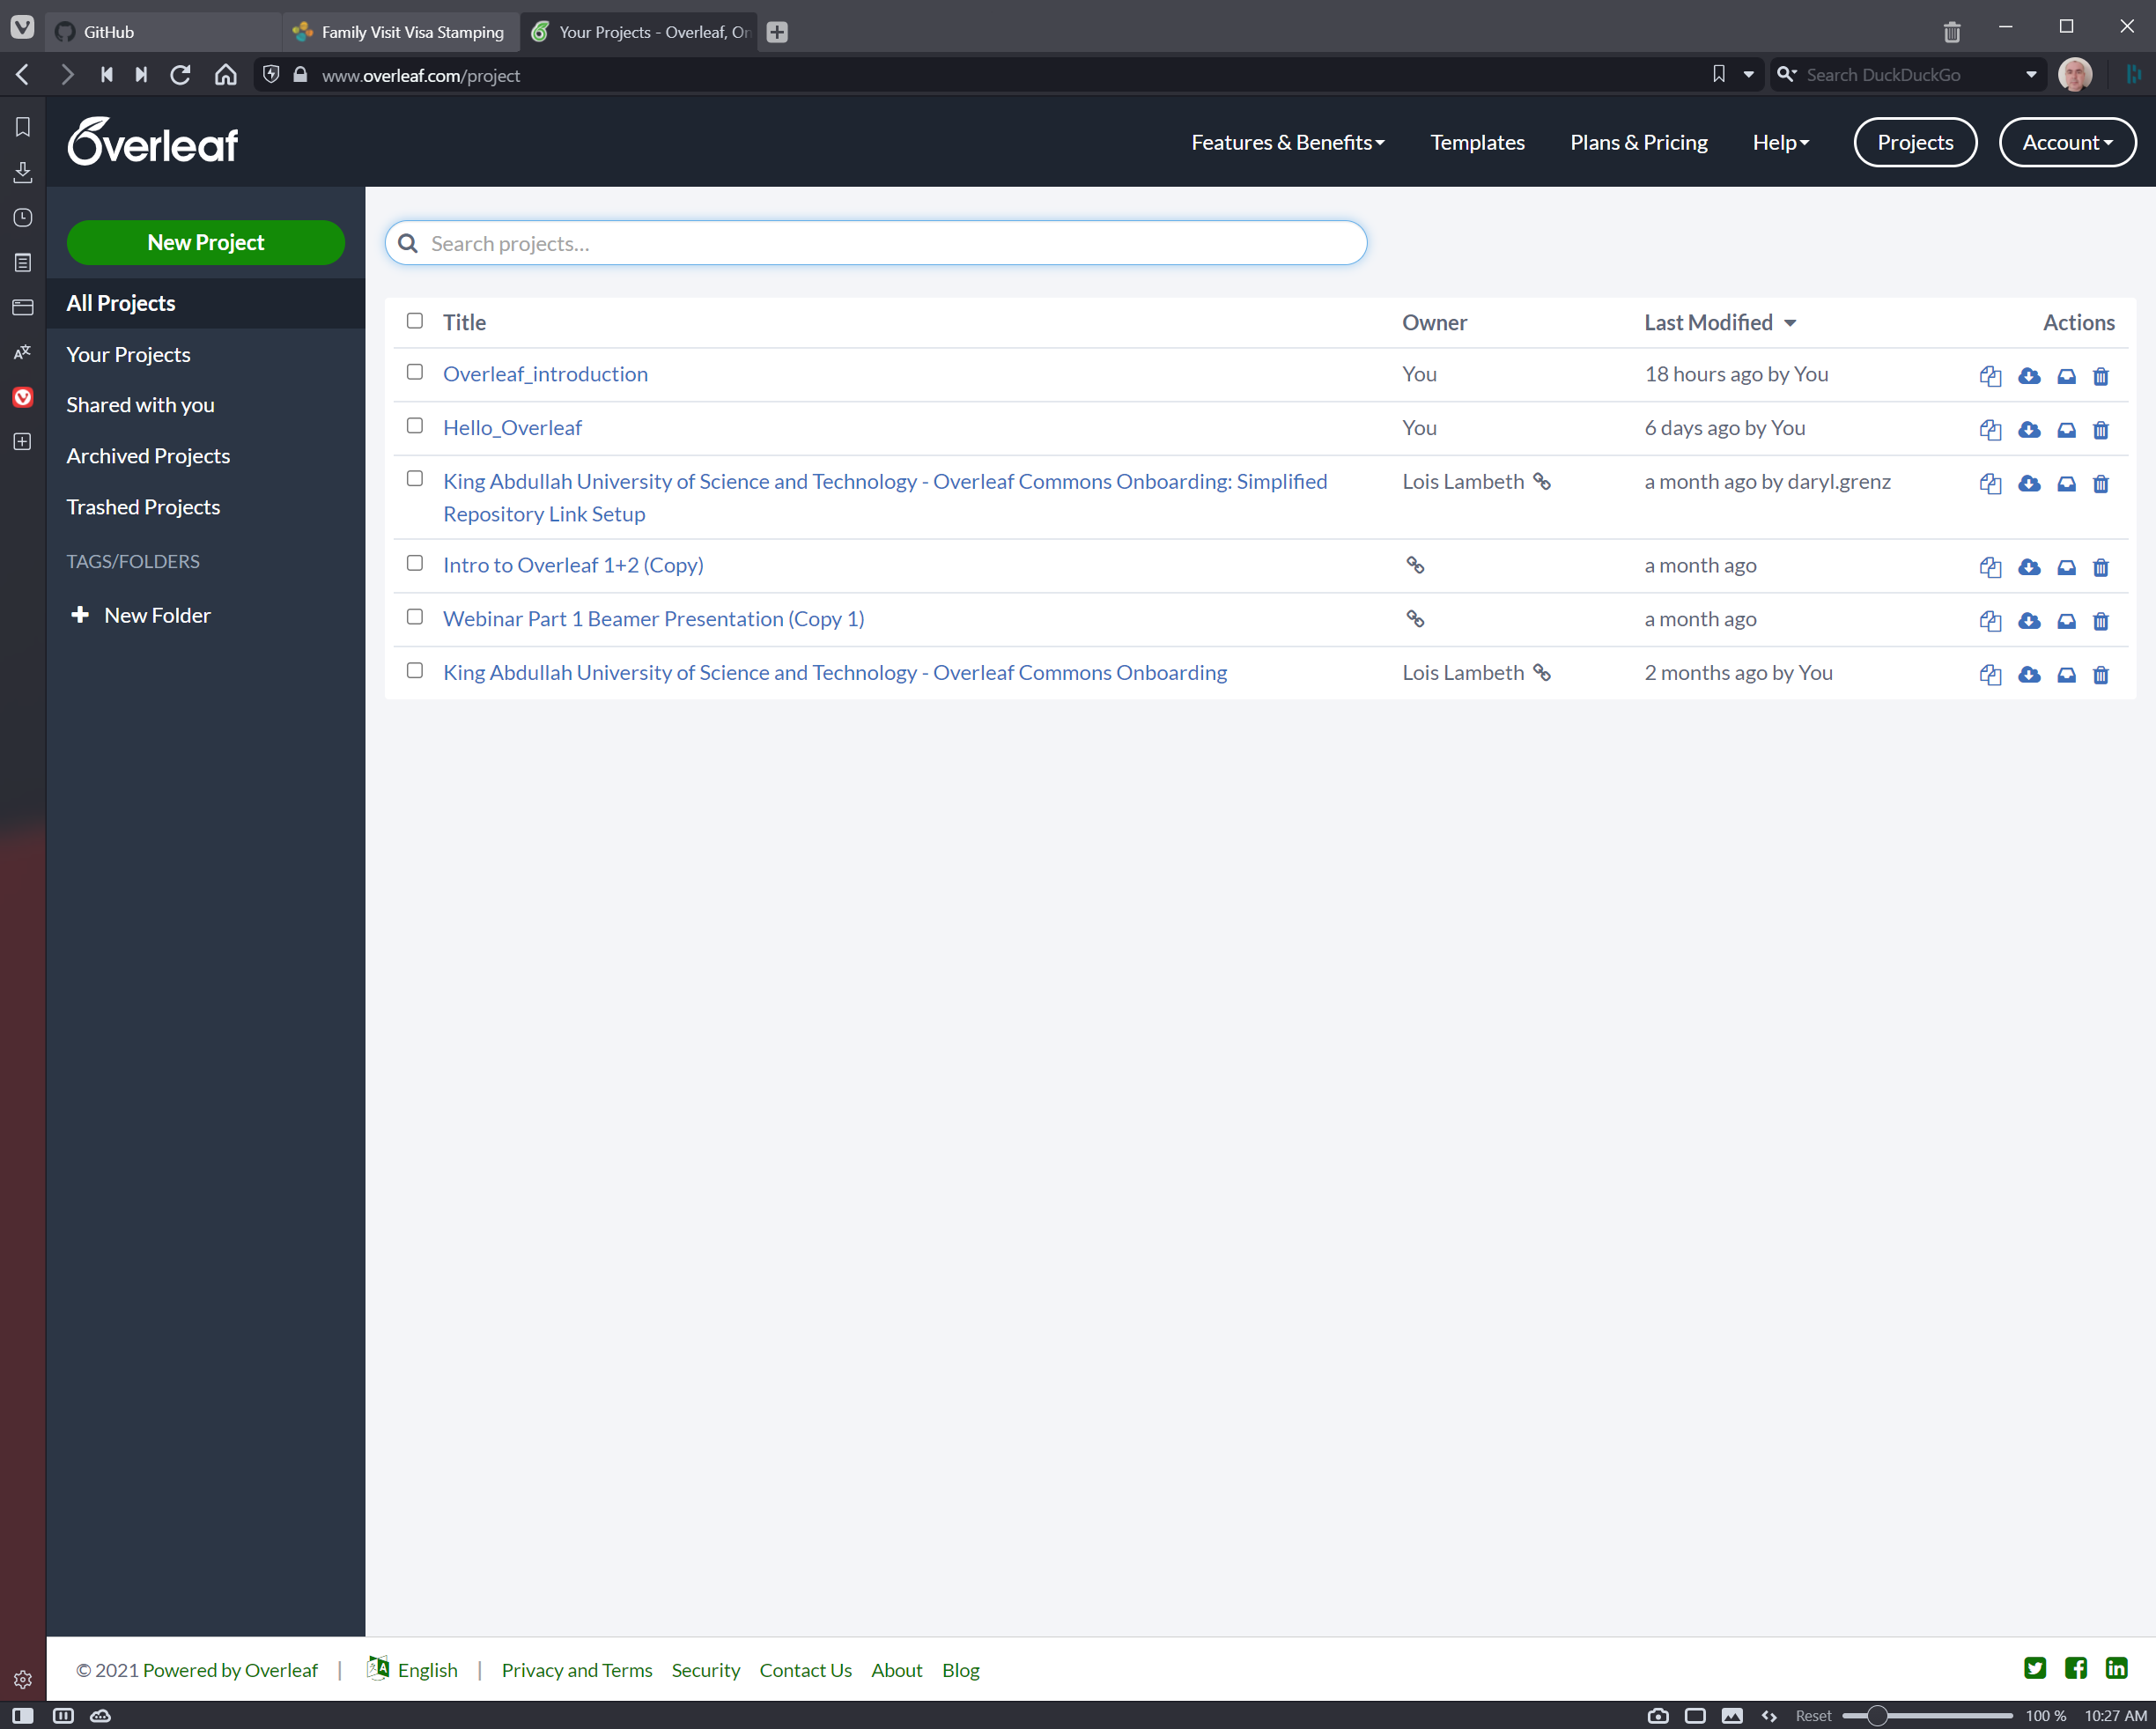
\includegraphics[scale=0.18]{images/overleaf_projects_view.png}
        %\caption{Caption}
        \label{fig:projects_overview}
    \end{figure}
\end{frame}

\begin{frame}{Split or Full Screen}
    Switching between split and full screen.
    \begin{figure}
        \centering
        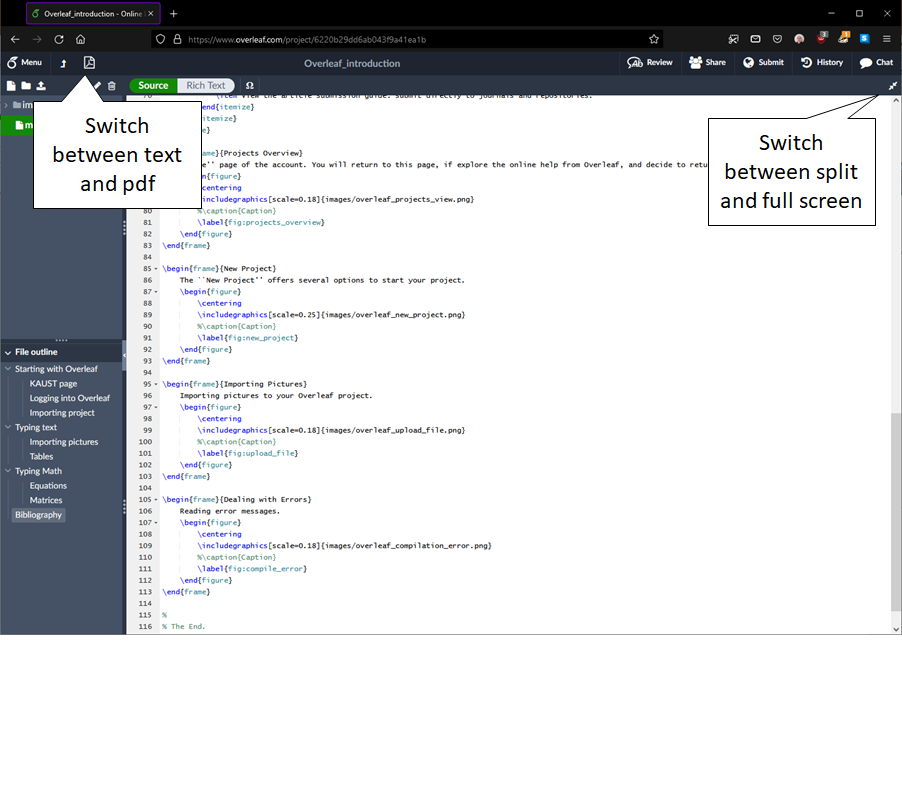
\includegraphics[scale=0.35]{images/overleaf_single_split_screen.png}
        %\caption{Caption}
        \label{fig:split_full_screen}
    \end{figure}
\end{frame}

\begin{frame}{New Project}
    The ``New Project'' offers several options to start your project.
    \begin{figure}
        \centering
        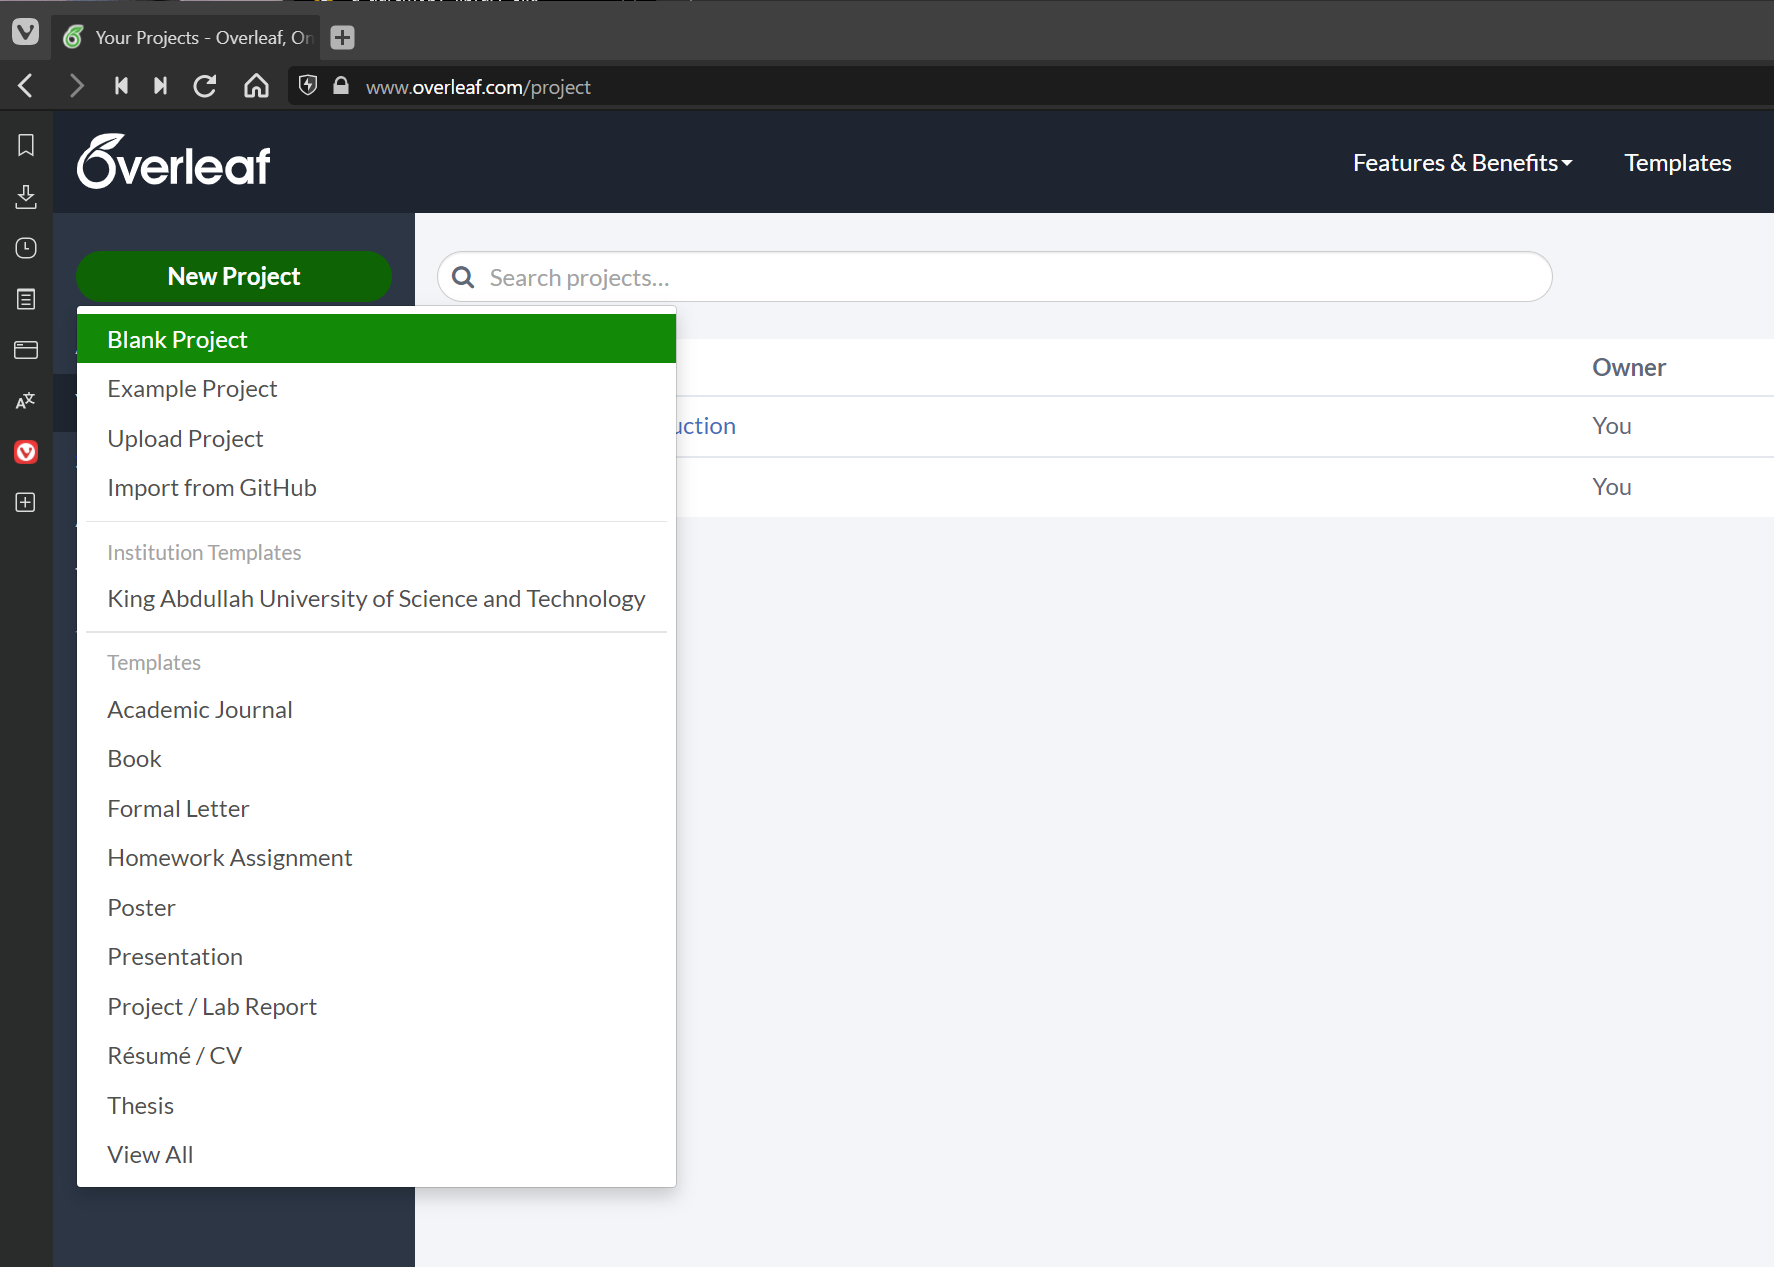
\includegraphics[scale=0.25]{images/overleaf_new_project.png}
        %\caption{Caption}
        \label{fig:new_project}
    \end{figure}
\end{frame}

\begin{frame}{Document Structure}
    Structure of a \LaTeX{} document. 
    \begin{figure}
        \centering
        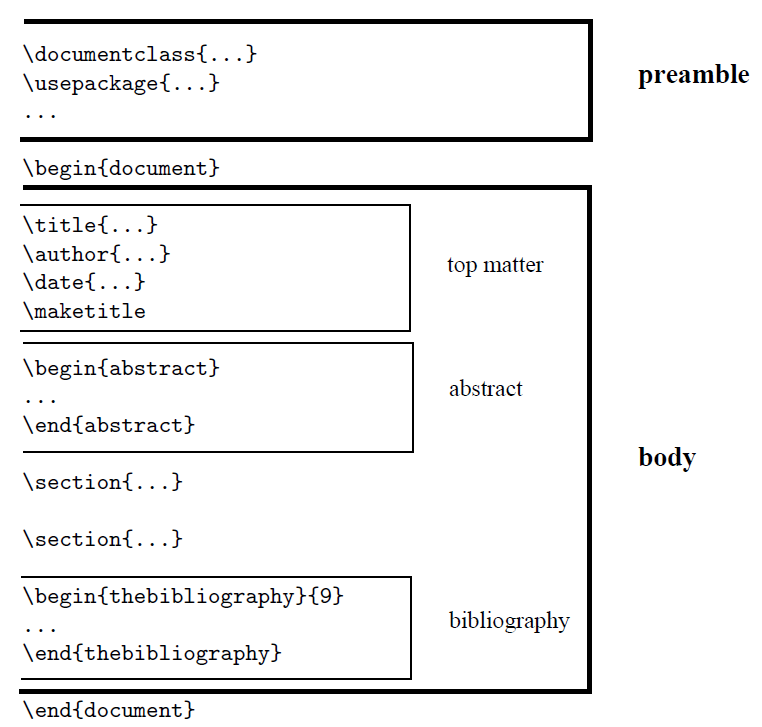
\includegraphics[scale=0.4]{images/latex_structure.png}
        %\caption{Caption}
        \label{fig:latexStruct}
    \end{figure}
\end{frame}

\begin{frame}[fragile]
\frametitle{The Preamble and Top Matter}
    The preamble and top matter of the document
    \begin{itemize}
        \item The \verb|\documentclass[parameter]{class}| command marks the beginning of the document. 
        \begin{itemize}
            \item Parameter (optional): font and paper size, like \texttt{10pt} or \texttt{a4paper}
            \item Class: the class of the document \textit{book, report, article, letter}, etc.  
            \item For example, the KAUST template document class
        \end{itemize}\small
        \begin{verbatim}
\documentclass[onecolumn, 12 pt, doublespace, fullpage, a4paper]{report}
        \end{verbatim}
        \item To combine more then one author use \verb|\and|, like \verb|\author{John \and Mary}|.
        \item You can control the date that is displayed by giving an explicit date, like \verb|\date{1st January 1970}|, or \verb|\date{\today}|, or \verb|\date{}| for no date.
    \end{itemize}
\end{frame}

\begin{frame}[fragile]
\frametitle{Working with Text}
    \begin{itemize}
        \item Several levels of sectioning: section, subsection, subsubsection, etc.
        \item Several font families
    \end{itemize}
    \medskip
    \small
    \begin{tabular}{l p{0.6\linewidth} }
         \textbf{Specifier} &  \textbf{Switches To}\\ \hline
         \verb|\textnormal{}|  & normal document text\\
         \verb|\emph{}| & \emph{emphasis}\\
         \verb|\texttt{}| & \texttt{Typewriter style font family}\\
         \verb|\textit{}| & \textit{italic text}\\
         \verb|\textbf{}| & \textbf{bold text}\\
         \verb|\textrm{}| & \textrm{Roman font family}\\
         \verb|\textsf{}| & \textsf{Sans-serif font family}\\         
    \end{tabular}
    \normalsize
\end{frame}

% \begin{frame}
% \frametitle{Working with Lists}

%     Using lists in \LaTeX{}
%     \begin{itemize}
%         \item We have the bullet list (\textit{itemize})
%     \end{itemize}
%     \begin{enumerate}
%         \item We have numbered list (\textit{enumerate})
%     \end{enumerate}
%     There is also a kind of list called ``description'', where the \textit{item} is highlighted. 
%     \begin{description}
%         \item[itemize:] is an unordered list. 
%         \item[enumerate:] is an ordered list
%     \end{description}
%     You can combine the lists creating nested lists.
% \end{frame}

\begin{frame}[fragile]
\frametitle{Example of Lists}
    \begin{columns}
        \begin{column}{0.5\textwidth}
        \scriptsize
        \begin{verbatim}
\begin{itemize}
    \item We have the bullet list
    \begin{itemize}
        \item A nested list
    \end{itemize}
\end{itemize}
\begin{enumerate}
    \item We have numbered list
    \begin{enumerate}
        \item Another nested list
    \end{enumerate}
\end{enumerate}
\begin{description}
    \item[itemize:] is an unordered list
    \item[enumerate:] is an ordered list
\end{description}
        \end{verbatim}
        \normalsize
        \end{column}
            
        \begin{column}{0.5\textwidth}
\begin{itemize}
    \item We have the bullet list
    \begin{itemize}
        \item A nested list
    \end{itemize}
\end{itemize}
\begin{enumerate}
    \item We have numbered list
    \begin{enumerate}
        \item Another nested list
    \end{enumerate}
\end{enumerate}
\begin{description}
    \item[itemize:] is an unordered list
    \item[enumerate:] is an ordered list
\end{description}
        \end{column}
    \end{columns}
\end{frame}

\begin{frame}{Importing Pictures}
    Importing pictures to your Overleaf project.
    \begin{figure}
        \centering
        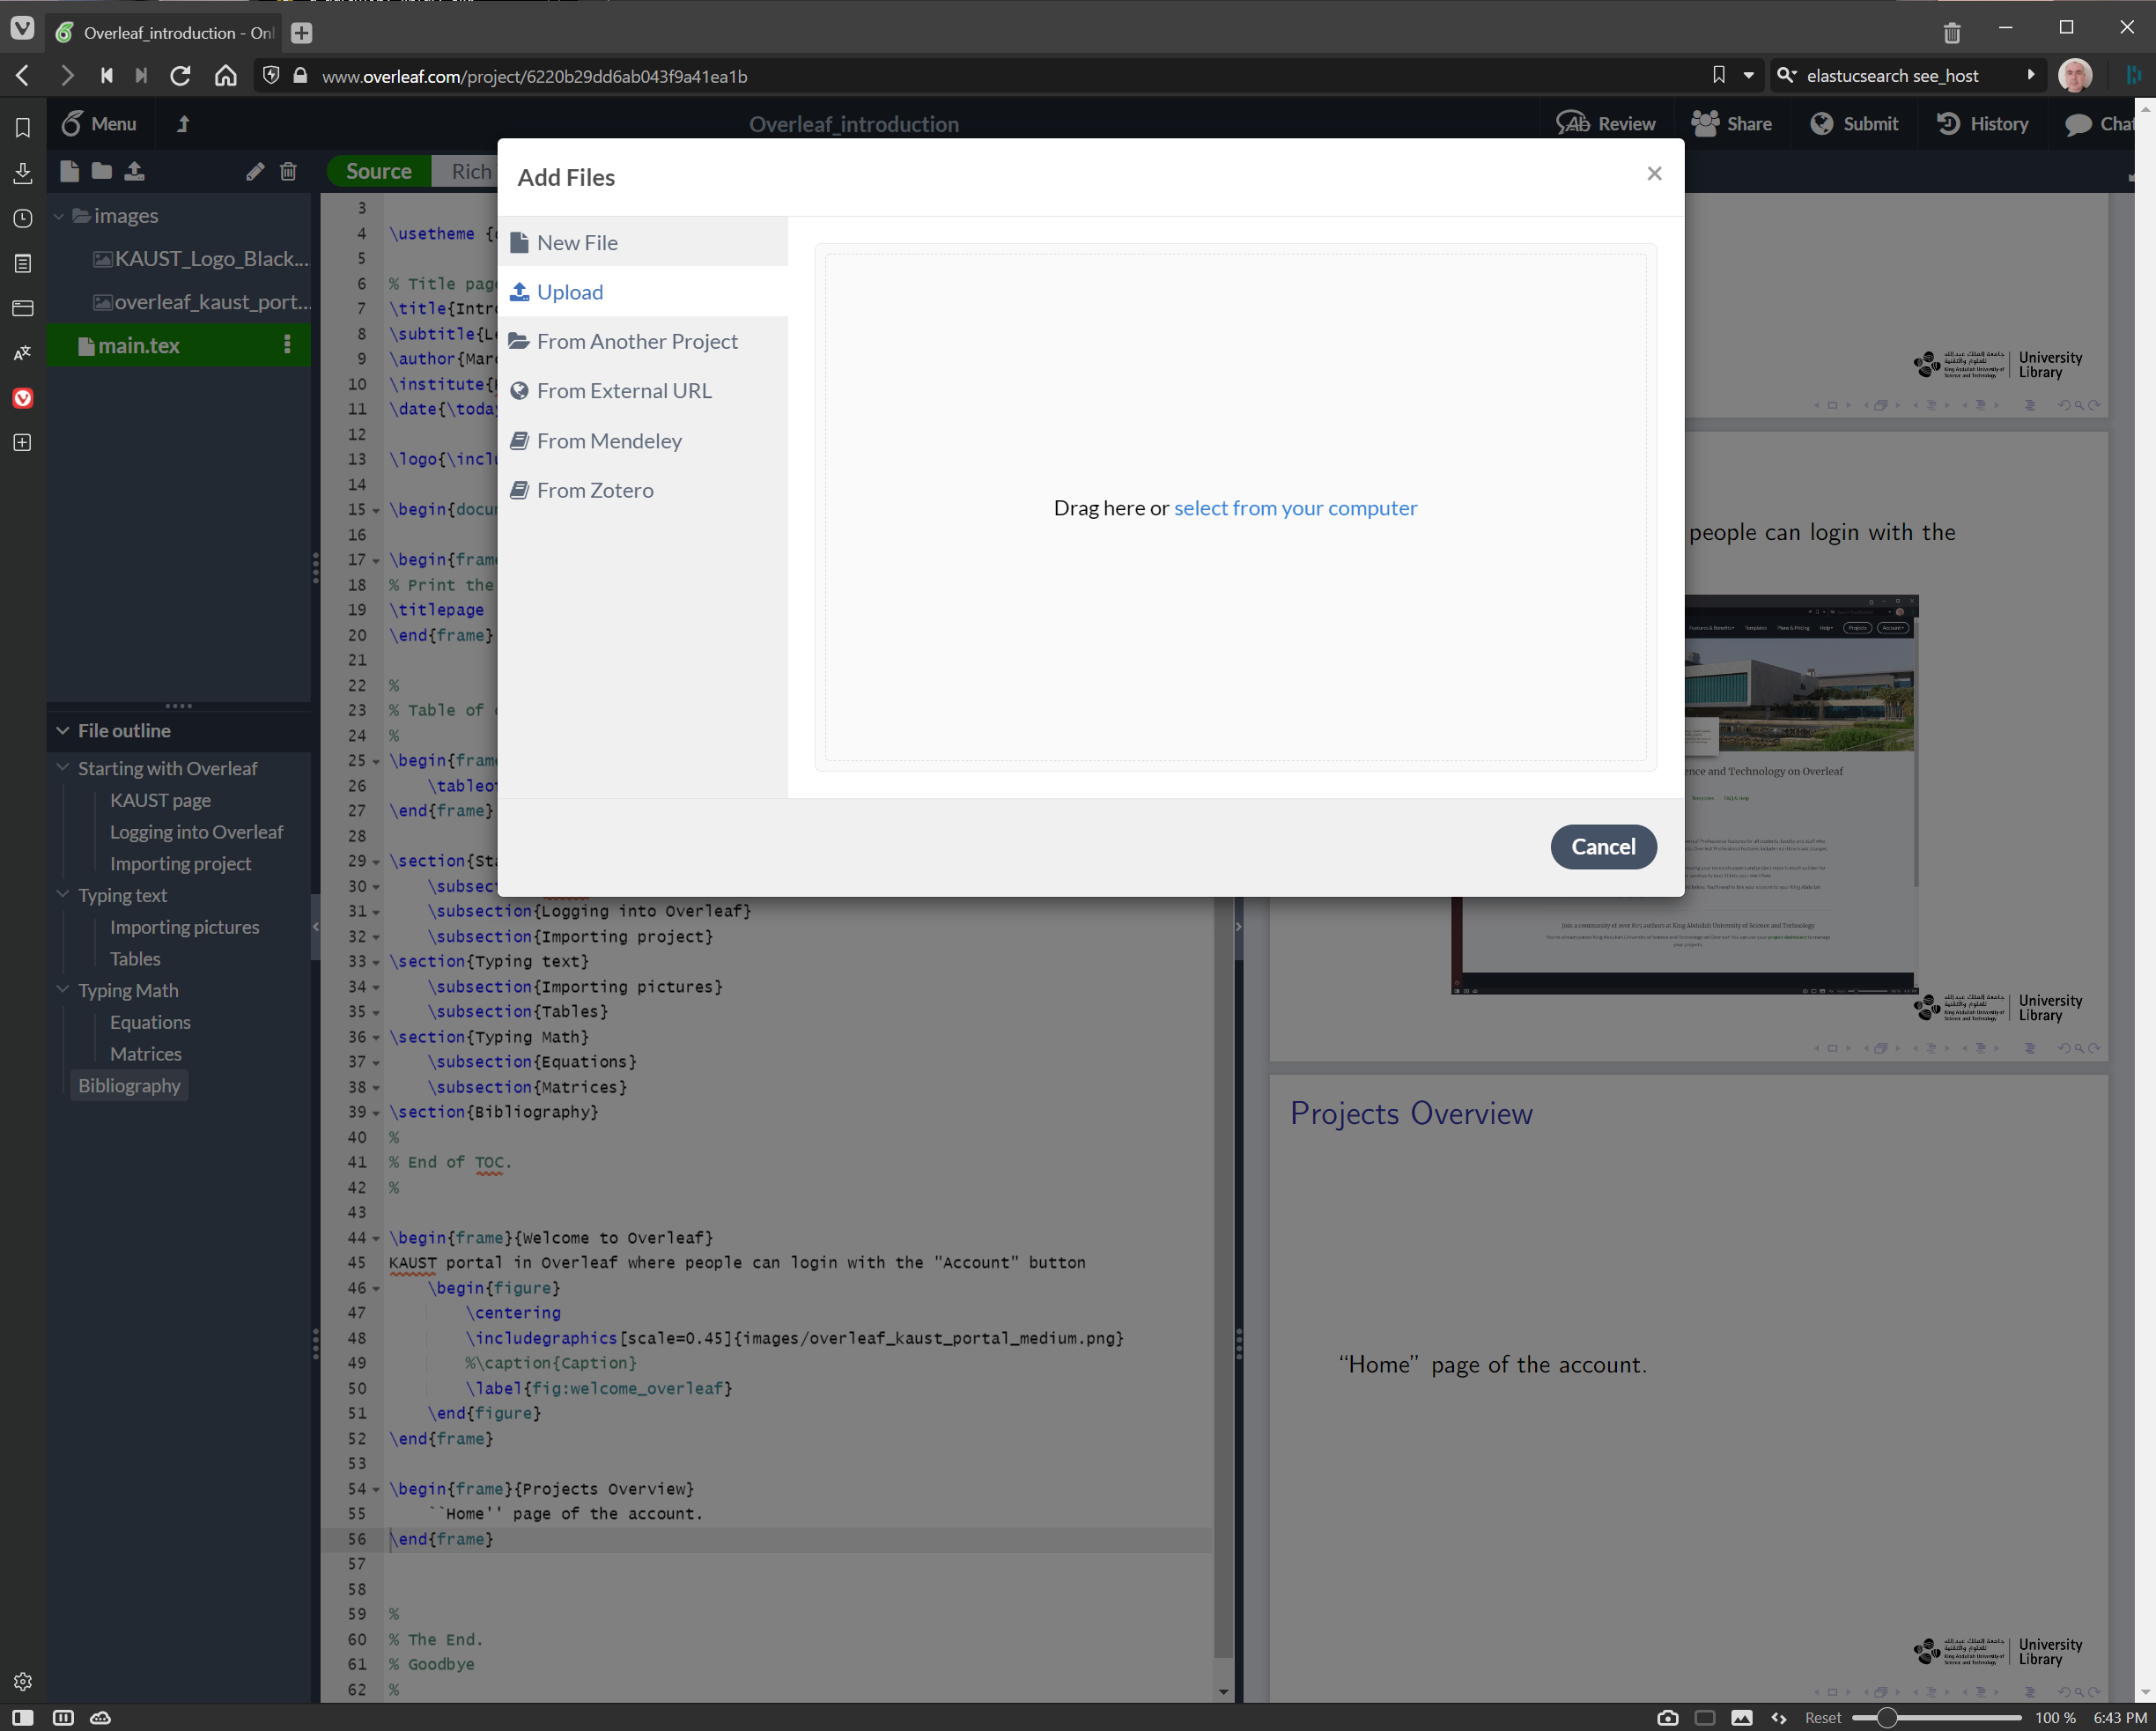
\includegraphics[scale=0.18]{images/overleaf_upload_file.png}
        %\caption{Caption}
        \label{fig:upload_file}
    \end{figure}
\end{frame}

\begin{frame}{Working with Pictures}
    Adding caption and setting the size of pictures
    \begin{itemize}
        \item Import the package \texttt{graphicx} to enable pictures in the document.
        \item You can specify the size of the pictures by scaling the pictures, like 10\% of the original size, or by explicitly setting dimension.
        \item Give ``hints'' of the picture placement, with $h$ for \textit{here} or $t$ for \textit{top}.
        \item Use the caption to explain the picture
        \item By labeling the picture, you can reference it later in the document.
    \end{itemize}
\end{frame}

\begin{frame}[fragile]
\frametitle{Example of Picture}

    \begin{columns}
        \begin{column}{0.5\textwidth}
        \tiny
        \begin{verbatim}
\begin{figure}[ht]
    \centering
    \includegraphics[width=0.5\textwidth] <break>
       {bombetoka_aster_23aug00_lrg}
    \caption{An Otherworldly-Looking Bombetoka Bay, 
      Madagascar}
    \label{fig:Bombetoka_Bay}
\end{figure}        
        \end{verbatim}
        \normalsize
        \end{column}
            
        \begin{column}{0.5\textwidth}
\begin{figure}[ht]
    \centering
    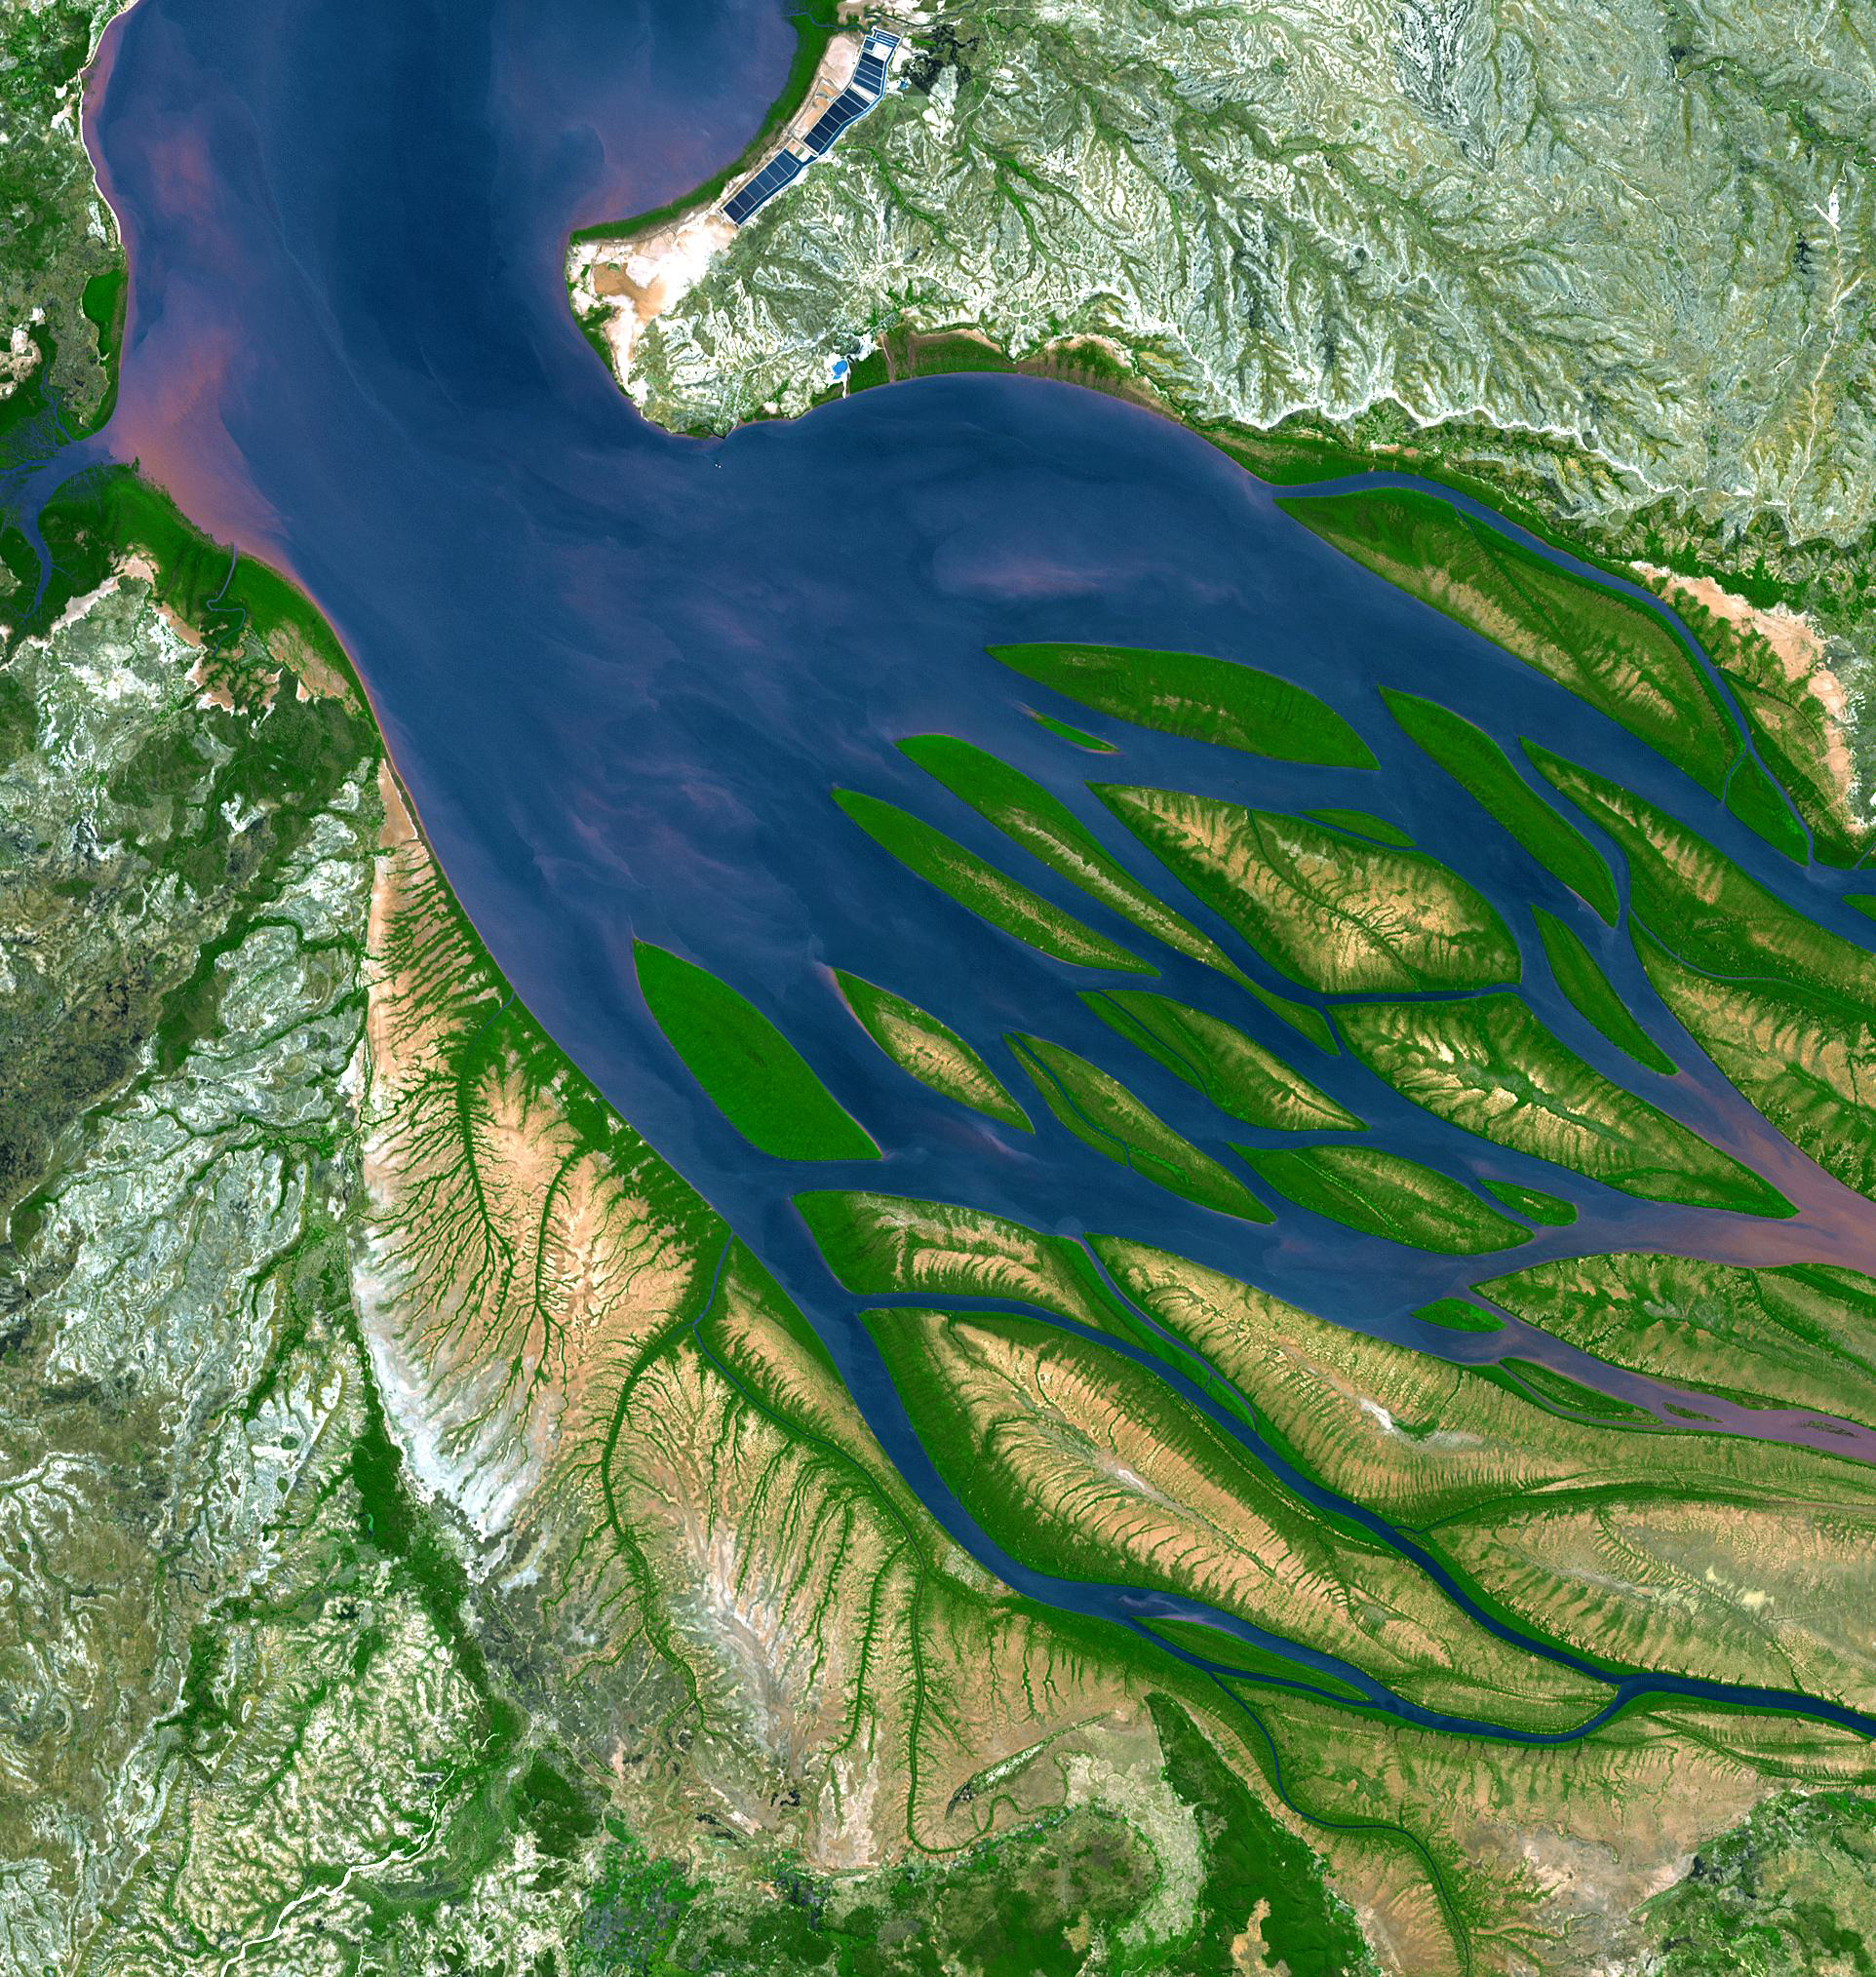
\includegraphics[width=0.5\textwidth]{images/bombetoka_aster_23aug00_lrg.jpg}
    \caption{An Otherworldly-Looking Bombetoka Bay, Madagascar}
    \label{fig:Bombetoka_Bay}
\end{figure}        
        \end{column}
    \end{columns}
    
\end{frame}

\begin{frame}[fragile]
\frametitle{Working with Equations}
    Here is where \LaTeX{} really shines! This is a huge topic, and we will cover only the basics.
    \begin{itemize}
        \item Load the packages \texttt{amssymb} and \texttt{latexsym}
        \item Inline math can type between the \verb|$...$|, like \verb|$\sqrt{5}$| will produce $\sqrt{5}$. 
        \item Equations will be in the equation environment
        \begin{verbatim}
            \begin{equation}
               x = \sqrt{5}
            \end{equation}
        \end{verbatim}
        \item Big and complex formulas require some planning
    \end{itemize}
\end{frame}

\begin{frame}[fragile]
\frametitle{Examples of Equations}

%
% Eq 1
%
\begin{columns}
    \tiny
    \begin{column}{0.5\textwidth}
        \begin{verbatim}
\begin{equation}\label{E:firstlnt}
\int_{O}^{\pi} \sin x \, dx = 2
\end{equation}
        \end{verbatim}
    \end{column}
    \begin{column}{0.5\textwidth}
\begin{equation}\label{E:firstlnt}
\int_{O}^{\pi} \sin x \, dx = 2
\end{equation}
    \end{column}
    \normalsize
\end{columns}

%
% Eq 2
% 
\begin{columns}
    \tiny
    \begin{column}{0.5\textwidth}
        \begin{verbatim}
\begin{align}
r^{2}  &= s^{2} + t^{2},               \label{E:Pyth}\\
2u + 1 &= v + w^{\alpha},              \label{E:alpha}\\
x      &= \frac{y + z}{\sqrt{s + 2u}}; \label{E:frac}
\end{align}
        \end{verbatim}
    \end{column}

    \begin{column}{0.5\textwidth}    
\begin{align}
r^{2}  &= s^{2} + t^{2},               \label{E:Pyth}\\
2u + 1 &= v + w^{\alpha},              \label{E:alpha}\\
x      &= \frac{y + z}{\sqrt{s + 2u}}; \label{E:frac}
\end{align}
    \end{column}
    \normalsize
\end{columns}

%
% Eq 3
%
\begin{columns}
    \tiny
    \begin{column}{0.5\textwidth}
        \begin{verbatim}
\[
f(x)=
\begin{cases}
-x^{2},     &\text{if $x < O$;}\\
\alpha + x, &\text{if $0 \leq x \leq 1$;}\\
x-{2},      &\text{otherwise.}
\end{cases}    
\]
        \end{verbatim}
    \end{column}
    \begin{column}{0.5\textwidth}    
\[
f(x)=
\begin{cases}
-x^{2},     &\text{if $x < O$;}\\
\alpha + x, &\text{if $0 \leq x \leq 1$;}\\
x-{2},      &\text{otherwise.}
\end{cases}    
\]
    \end{column}
    \normalsize
\end{columns}

%
% Eq 4
%
\begin{columns}
    \tiny
    \begin{column}{0.5\textwidth}
        \begin{verbatim}
\[
\overbrace{a + b + \cdots + z}^{n}
\]
        \end{verbatim}
    \end{column}
    \begin{column}{0.5\textwidth}
\[
\overbrace{a + b + \cdots + z}^{n}
\]
    \end{column}
    \normalsize
\end{columns}

  
\end{frame}

\begin{frame}[fragile]
\frametitle{Working with Tables}
    Creating tables in \LaTeX
    \begin{itemize}
        \item Start simple with the \texttt{tabular} environment
        \item Define the alignment of columns, left (\texttt{l}), center (\texttt{c}) or right (\texttt{r}).
        \item Then add borders with \verb|\hline| for horizontal lines and for vertical lines, define together with the header, like 
\begin{verbatim}
{||c c c c||}    
\end{verbatim}
        \item Add the \texttt{table} environment 
        \item Finally finish the table environment by defining the adding caption and label.
    \end{itemize}
\end{frame}

\begin{frame}[fragile]
\frametitle{Example Table}
    \begin{columns}
        \tiny
        \begin{column}{0.5\textwidth}
            \begin{verbatim}
\begin{table}[h!]
    \centering
    \begin{tabular}{||c c c c||} 
     \hline
     Col1 & Col2 & Col2 & Col3 \\ [0.5ex] 
     \hline\hline
     1 & 6 & 87837 & 787 \\ 
     2 & 7 & 78 & 5415 \\
     3 & 545 & 778 & 7507 \\
     4 & 545 & 18744 & 7560 \\
     5 & 88 & 788 & 6344 \\ [1ex] 
     \hline
    \end{tabular}
    \caption{Table to test captions and labels}
    \label{table:data}
\end{table}
            \end{verbatim}
        \end{column}
            
        \begin{column}{0.5\textwidth}

            \begin{table}[h!]
                \centering
                \begin{tabular}{||c c c c||} 
                 \hline
                 Col1 & Col2 & Col2 & Col3 \\ [0.5ex] 
                 \hline\hline
                 1 & 6 & 87837 & 787 \\ 
                 2 & 7 & 78 & 5415 \\
                 3 & 545 & 778 & 7507 \\
                 4 & 545 & 18744 & 7560 \\
                 5 & 88 & 788 & 6344 \\ [1ex] 
                 \hline
                \end{tabular}
                \caption{Table to test captions and labels}
                \label{table:data}
            \end{table}    
        \end{column}
        \normalsize
        
    \end{columns}

\end{frame}

\begin{frame}[fragile]
\frametitle{Bibliography}

    \begin{itemize}
        \item Add the package \texttt{biblatex}
        \item Specify the file with the bibliography entries
        \item You reference the citation with \verb|\cite{...}|
        \item Several supported entries: books, articles, patents, proceedings, conference, etc
        \item Several styles of bibliography are supported: numeric, alphabetic authoryear, etc
        \item Specific bibliography style for some magazines like Nature, IEEE, Science, and others.
        \item Where do you want the bibliography list to appear, add the command \verb|\printbibliography|.        
    \end{itemize}
    
\end{frame}

\begin{frame}{Comparing Versions}
    You can compare different versions of the document using the ``History''.
    \begin{figure}
        \centering
        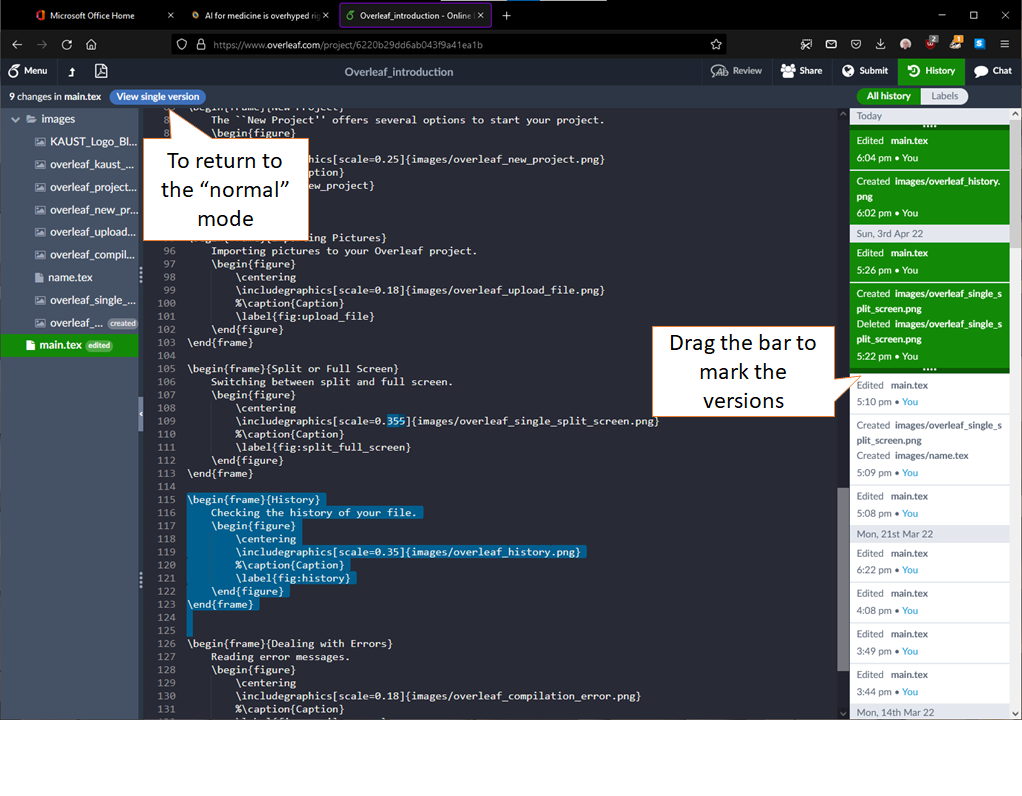
\includegraphics[scale=0.3]{images/overleaf_history_compare_2.png}
        %\caption{Caption}
        \label{fig:history_compare}
    \end{figure}
\end{frame}

\begin{frame}{Using Tags}
    Tag your versions to mark special versions.
    \begin{figure}
        \centering
        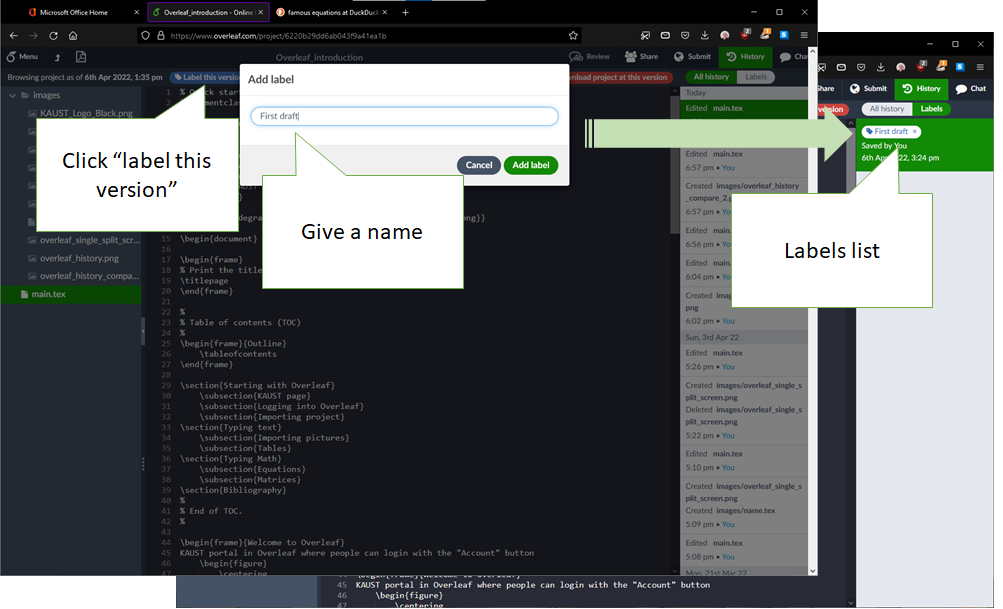
\includegraphics[scale=0.35]{images/overleaf_hist_tag_3.png}
        %\caption{Caption}
        \label{fig:history_tags}
    \end{figure}
\end{frame}

\begin{frame}[fragile]
\frametitle{Working Offline}

    \begin{itemize}
        \item Working offline or with a collaborator that doesn't have Overleaf.
        \item Options for Dropbox, Git and Github.
        \item Using Github as example
        \begin{enumerate}
            \item Create the project in Github
            \item Import into Overleaf as new project
            \item Remember to synchronize the two projects!! (Not automatic)
        \end{enumerate}
    \end{itemize}
\end{frame}

\begin{frame}{Dealing with Errors}
    Reading error messages.
    \begin{figure}
        \centering
        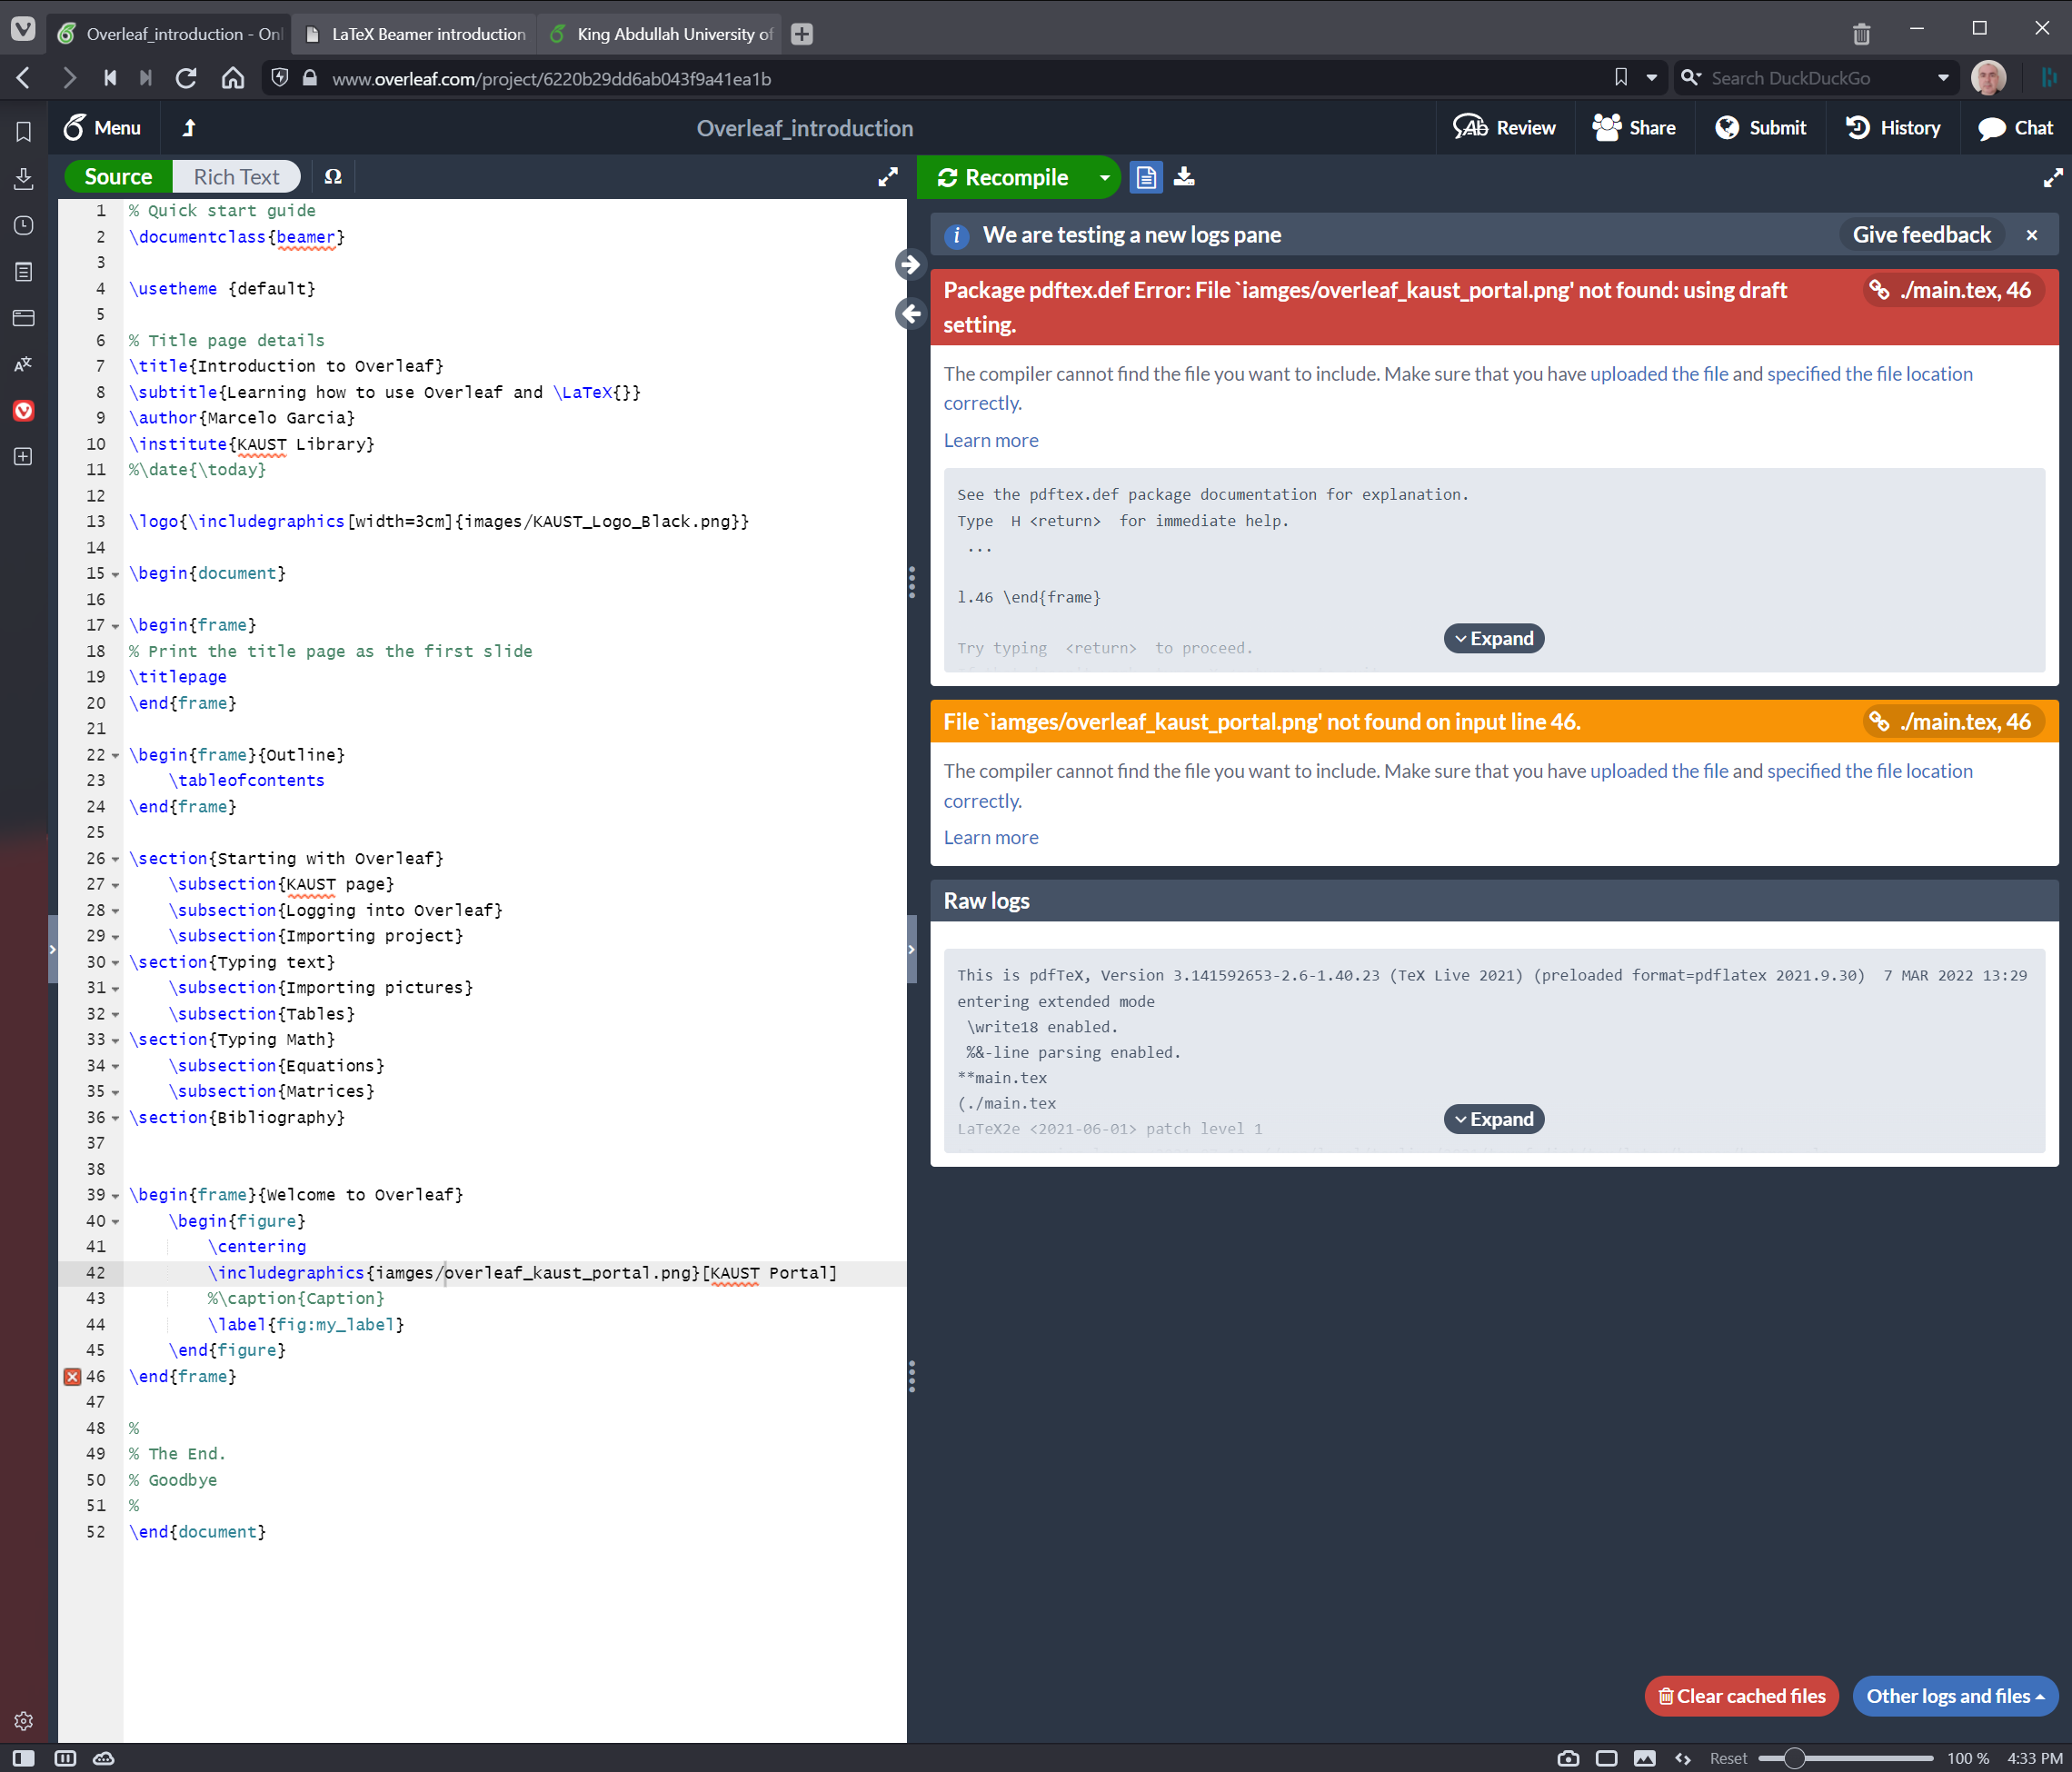
\includegraphics[scale=0.18]{images/overleaf_compilation_error.png}
        %\caption{Caption}
        \label{fig:compile_error}
    \end{figure}
\end{frame}

% 
% The End.
% Goodbye
%
\end{document}